\documentclass[]{article}
\usepackage[latin1]{inputenc}
\usepackage{ragged2e}
\AtBeginDocument{\RaggedRight}
\usepackage{amsmath}
\usepackage{amssymb}
\usepackage{amsthm}
\renewcommand{\labelitemi}{\color{MPIIblue} $\blacktriangleright$}
\usepackage{rotating}
\usepackage{latexsym}
\usepackage{graphicx}
\usepackage{wasysym}
\usepackage{multirow}
\graphicspath{{../Stutz2019CVPR/}}
\usepackage{url}
\usepackage{calc}
\usepackage[
    paperheight=20cm,
    paperwidth=35.5cm,
    left=3mm,
    right=3mm,
    top=2mm,
    bottom=2mm,
    includehead,
    headheight=17.5mm,
]{geometry}
\usepackage{fancyhdr}
\usepackage{parskip}
\usepackage{tikz}
\usetikzlibrary{math}
\usepackage{tikz-3dplot}
\usepackage{pgfplots}
\usetikzlibrary{calc}
\usetikzlibrary{shadings,shadows}
\usepackage{xcolor}
\usepackage{tcolorbox}
\tcbuselibrary{skins,breakable}
\usepackage[backend=bibtex,style=numeric]{biblatex}

\pagestyle{fancy}
\makeatletter
\def\headrule{}
\def\footrule{}
\makeatother
\lfoot{ %
    %\hspace*{0.5mm}
    %\raisebox{14.5mm}{
\includegraphics[height=14mm]{gfx/mpilogo-inf-narrow}}
}
\cfoot{}
\rfoot{ %
    %\raisebox{16mm}{
\includegraphics[height=12mm]{gfx/UT_WBMW_Rot_RGB}}
}
\lhead{%
	\hspace*{2mm}\raisebox{0mm}{
\includegraphics[height=15mm]{mpilogo-inf-narrow}}\hspace*{2.5mm}
}
\chead{%
    \vspace*{2mm}
    \hspace*{1.5mm}{\bf\LARGE Relating Adversarially Robust Generalization to Flat Minima}\\[3mm]
    \hspace*{1.5mm}{\Large David Stutz, Matthias Hein, Bernt Schiele}
}
\rhead{%
    \raisebox{0mm}{
\includegraphics[height=15mm]{UT_WBMW_Rot_RGB}}\hspace*{2mm}
}

\bibliography{bibliography}

\renewcommand{\rmdefault}{phv}
\renewcommand{\sfdefault}{phv}
\renewcommand{\ttdefault}{pcr}

\definecolor{MPIIblue}{RGB}{0,51,93}
\definecolor{MPIIlightblue}{RGB}{103,133,158} % 67859E
\definecolor{MPIIorange}{RGB}{200,91,15} % C85B0F
\definecolor{MPIIblack}{RGB}{46,46,46}
\definecolor{MPIIwhite}{RGB}{255,255,255}
\definecolor{MPIIdarkgray}{RGB}{123,123,123}
\definecolor{MPIIdarkergray}{RGB}{89,89,89}
\definecolor{MPIIgray}{RGB}{169,169,169}
\definecolor{MPIIlightgray}{RGB}{214,214,214}
\definecolor{MPIIlightergray}{RGB}{234,234,234}
\definecolor{MPIIgreen}{HTML}{327a2b} % 0.22,0.54, 0.19
\definecolor{MPIIred}{rgb}{0.65,0.23,0.25}
\definecolor{MPIIbeige}{rgb}{0.65,0.23,0.25}
\definecolor{MPIIpink}{HTML}{d36582}
\definecolor{MPIIteal}{HTML}{4d7c8a}
\definecolor{MPIIviolet}{HTML}{3c1642}
\definecolor{MPIIbrown}{HTML}{5a352a}
\definecolor{MPIIyellow}{HTML}{eee82c}
\definecolor{colorbrewer0}{RGB}{45,45,45}
\definecolor{colorbrewer1}{RGB}{228,26,28}
\definecolor{colorbrewer2}{RGB}{55,126,184}
\definecolor{colorbrewer3}{RGB}{77,175,74}
\definecolor{colorbrewer4}{RGB}{152,78,163}
\definecolor{colorbrewer5}{RGB}{255,127,0}
\definecolor{colorbrewer6}{RGB}{255,255,51}
\definecolor{colorbrewer7}{RGB}{166,86,40}
\definecolor{colorbrewer8}{RGB}{247,129,191}
\definecolor{colorbrewer9}{RGB}{153,153,153}
\definecolor{colorbrewer10}{RGB}{24,167,181}

\newenvironment{problem}[1]{%
    \tcolorbox[noparskip,frame hidden,boxrule=0.5mm,colframe=MPIIblue,
    colbacktitle=MPIIblue,coltitle=MPIIwhite,
    colback=MPIIwhite,
    titlerule=0mm,sharpish corners,no shadow,
    left=1.5mm,top=1.5mm,right=1.5mm,bottom=1mm,
    lefttitle=1.5mm,toptitle=2mm,righttitle=1.5mm,bottomtitle=2mm,
    title=#1]}%
{\endtcolorbox}
\newenvironment{related}[1]{%
    \tcolorbox[noparskip,frame hidden,boxrule=0.5mm,colframe=MPIIgray,
    colbacktitle=MPIIgray,coltitle=MPIIwhite,
    colback=MPIIwhite,
    titlerule=0mm,sharpish corners,no shadow,
    left=1.5mm,top=1.5mm,right=1.5mm,bottom=1mm,
    lefttitle=1.5mm,toptitle=2mm,righttitle=1.5mm,bottomtitle=2mm,
    title=#1]}%
{\endtcolorbox}
\newenvironment{method}[1]{%
    \tcolorbox[noparskip,frame hidden,boxrule=0.5mm,colframe=MPIIorange,
    colbacktitle=MPIIorange,coltitle=MPIIwhite,
    colback=MPIIwhite,
    titlerule=0mm,sharpish corners,no shadow,
    left=1.5mm,top=1.5mm,right=1.5mm,bottom=1mm,
    lefttitle=1.5mm,toptitle=2mm,righttitle=1.5mm,bottomtitle=2mm,
    title=#1]}%
{\endtcolorbox}
\newenvironment{data}[1]{%
    \tcolorbox[noparskip,frame hidden,boxrule=0.5mm,colframe=MPIIgray,
    colbacktitle=MPIIgray,coltitle=MPIIwhite,
    colback=MPIIwhite,
    titlerule=0mm,sharpish corners,no shadow,
    left=1.5mm,top=1.5mm,right=1.5mm,bottom=1mm,
    lefttitle=1.5mm,toptitle=2mm,righttitle=1.5mm,bottomtitle=2mm,
    title=#1]}%
{\endtcolorbox}
\newenvironment{results}[1]{%
    \tcolorbox[noparskip,frame hidden,boxrule=0.5mm,colframe=MPIIlightgray,
    colbacktitle=MPIIlightgray,coltitle=MPIIblue,
    colback=MPIIwhite,
    titlerule=0mm,sharpish corners,no shadow,
    left=1.5mm,top=1.5mm,right=1.5mm,bottom=1mm,
    lefttitle=1.5mm,toptitle=1.05mm,righttitle=1.5mm,bottomtitle=1.05mm,
    title=#1]}%
{\endtcolorbox}
\newenvironment{moreresults}[1]{%
	\tcolorbox[noparskip,frame hidden,boxrule=0.5mm,colframe=MPIIlightgray,
	colbacktitle=MPIIwhite,coltitle=MPIIblue,
	colback=MPIIwhite,
	titlerule=0.5mm,sharpish corners,no shadow,
	left=1.5mm,top=1.5mm,right=1.5mm,bottom=1mm,
	lefttitle=1mm,toptitle=0.5mm,righttitle=1mm,bottomtitle=0.25mm,
	title=#1]}%
{\endtcolorbox}
\newenvironment{code}[1]{%
    \tcolorbox[noparskip,frame hidden,boxrule=0mm,colframe=MPIIwhite,
    colback=MPIIorange,coltext=MPIIwhite,
    titlerule=0mm,sharpish corners,no shadow,
    left=2.5mm,top=2.5mm,right=2.5mm,bottom=2.5mm,
    lefttitle=1.5mm,toptitle=2mm,righttitle=1.5mm,bottomtitle=2mm,
    title=#1]}%
{\endtcolorbox}
\newenvironment{references}[1]{%
    \tcolorbox[noparskip,frame hidden,boxrule=0.5mm,colframe=MPIIlightgray,
    colbacktitle=MPIIwhite,coltitle=MPIIdarkergray,
    colback=MPIIwhite,
    titlerule=0mm,sharpish corners,no shadow,
    left=1.5mm,top=0.25mm,right=1.5mm,bottom=0.5mm,
    lefttitle=1.5mm,toptitle=2mm,righttitle=1.5mm,bottomtitle=2mm,
    title=#1]}%
{\endtcolorbox}

\begin{document}
	\vspace*{-10mm}
	\begin{minipage}[t]{0.32\textwidth}
	     \strut\vspace*{-\baselineskip} % !
	     
	     \begin{results}{\bf\large Robust Overfitting}
			\large = test robustness eventually increases in training \cite{RiceICML2020}.\\[1px]
			{\color{MPIIblue}$\RHD$} Worst in robust loss on mis-classified examples.
			
			\vspace*{6px}
			\begin{minipage}[t]{0.49\textwidth}
				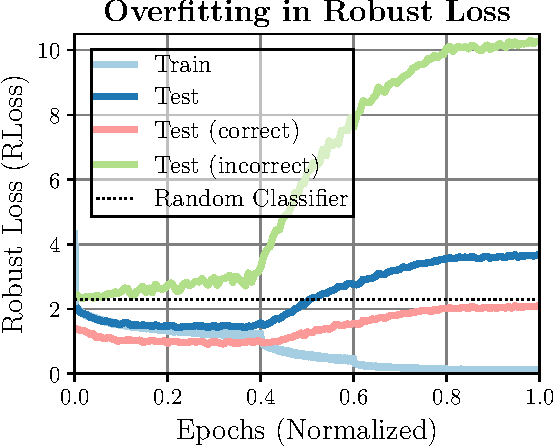
\includegraphics[width=\textwidth]{../paper/plots_short_introduction_overfitting1.pdf}
			\end{minipage}
			\hfill
			\begin{minipage}[t]{0.49\textwidth}
				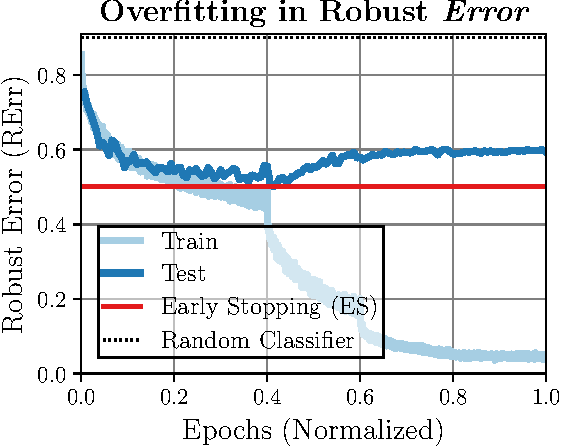
\includegraphics[width=\textwidth]{../paper/plots_short_introduction_overfitting2.pdf}
			\end{minipage}
	     \end{results}
	     
	     \begin{results}{\bf\large Robust Flatness}
     	     {\large Adapted average- and worst-case flatness \cite{KeskarICLR2017,NeyshaburNIPS2017}:}
     	     
     	     \vspace*{0px}
     	     \begin{minipage}[t]{0.26\textwidth}
     	     	\vspace*{0px}
     	     	
     	     	\fbox{
     	     		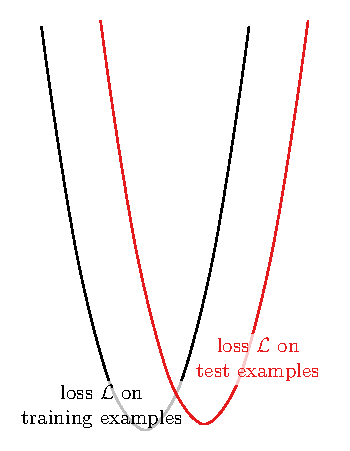
\includegraphics[width=\textwidth]{../paper/fig_main_illustration2.pdf}
     	     	}
     	     \end{minipage}
     	     \hfill
     	     \begin{minipage}[t]{0.68\textwidth}
     	     	\vspace*{-4px}
     	     	
     	     	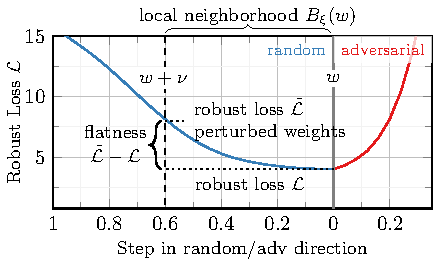
\includegraphics[width=\textwidth]{../paper/fig_main_illustration1.pdf}
     	     \end{minipage}
  	     \end{results}
  	     
  	     \begin{moreresults}{}
  	     	 \large {Average-case flatness measure:}
	  	     \begin{align}
     	     	\begin{split}
     	     		\underbrace{\mathbb{E}_{\nu}[\max\limits_{\|\delta\|_\infty \leq \epsilon} \mathcal{L}(f(x{+}\delta; w{+}\nu), y)]}_{\text{``perturbed'' \textit{robust} loss }\tilde{\mathcal{L}}} - \underbrace{\max\limits_{\|\delta\|_\infty \leq \epsilon} \mathcal{L}(f(x{+}\delta;w), y)}_{\text{reference \textit{robust} loss }\mathcal{L}}\notag
     	     	\end{split}
	  	     \end{align}
  	     \end{moreresults}
	 \end{minipage}
	 \hfill
    \begin{minipage}[t]{0.34\textwidth}
        \strut\vspace*{-\baselineskip} % !
        
        \begin{problem}{\bfseries\large Problem}
        	\large How do methods \textbf{improve robustness} \& avoid overfitting?\\[1px]
        	{\color{MPIIblue}$\RHD$} Do they find ``better'' = \textbf{flatter minima}?
        \end{problem}
        
        \begin{method}{\bfseries\large Contributions}
        	\large Clear \textbf{correlation} between \textbf{flatness and robustness}:
        	
        	\vspace*{8px}
        	\begin{center}
        		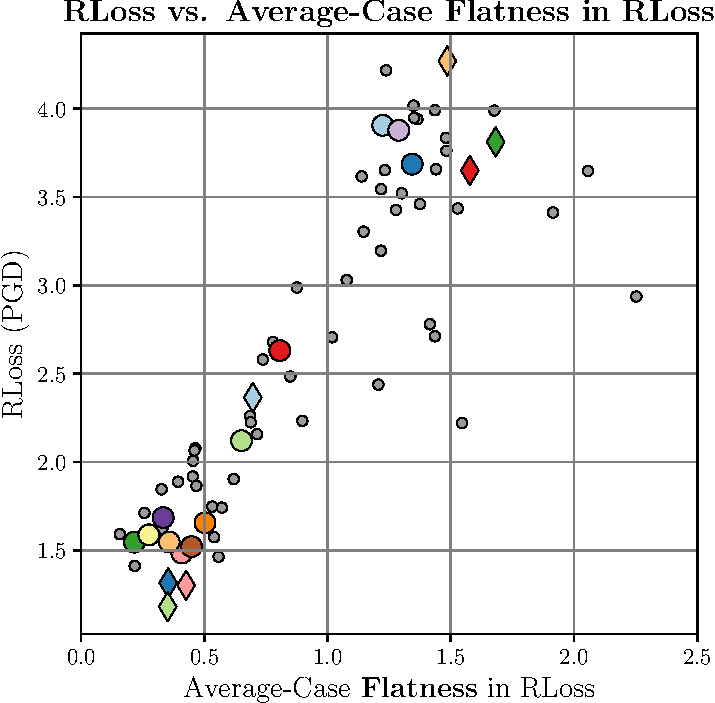
\includegraphics[width=0.65\textwidth]{../paper/plots_main_flatness_correlation_seq_loss.pdf}
        		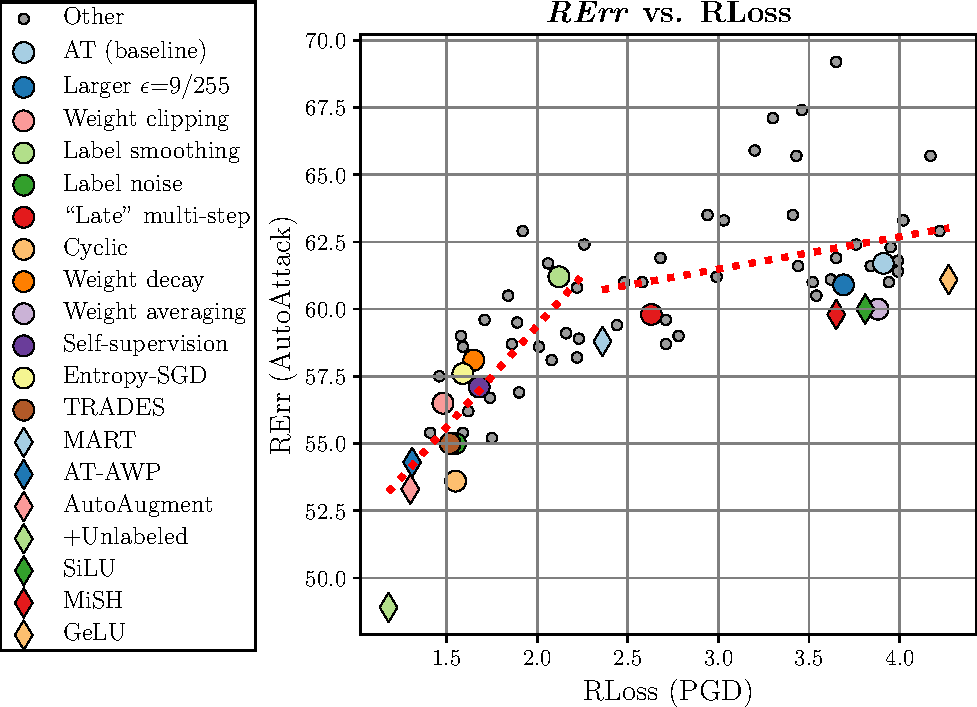
\includegraphics[width=0.25\textwidth,clip,trim={0 0 12cm 0}]{../paper/plots_main_loss_error.pdf}
        	\end{center}
        \end{method}
    
   		\begin{code}{}
		 	\large
		 	Paper and Code: \bf\url{davidstutz.de/flatness}
		\end{code}
   
        \begin{references}{}
            \vspace*{0.325mm}
	        \AtNextBibliography{\fontsize{8}{10}\selectfont}
	        {\begingroup
	            \color{MPIIdarkergray}
	            \renewcommand{\section}[2]{}%
	            \printbibliography
	            \endgroup}
	    \end{references}
    \end{minipage}
    \hfill
    \begin{minipage}[t]{0.32\textwidth}
        \strut\vspace*{-\baselineskip} % !
        
		\begin{results}{\bf\large Flatness Throughout Training}
		
			\begin{center}
				\begin{minipage}[t]{0.475\textwidth}
					\vspace*{0px}
					
					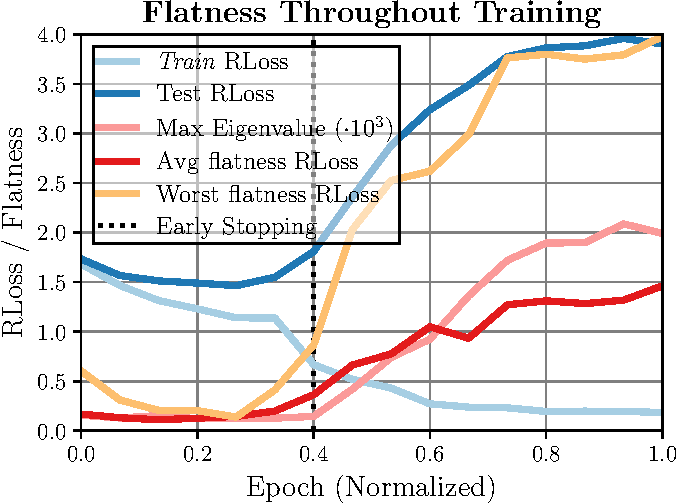
\includegraphics[width=1.025\textwidth]{../paper/plots_main_flatness_epochs}
				\end{minipage}
				\begin{minipage}[t]{0.015\textwidth}
					\vspace*{0px}
					
					\hspace*{4px}{\color{black!75}\rule{0.65px}{3.5cm}}
				\end{minipage}
				\begin{minipage}[t]{0.2\textwidth}
					\vspace*{0px}
					
					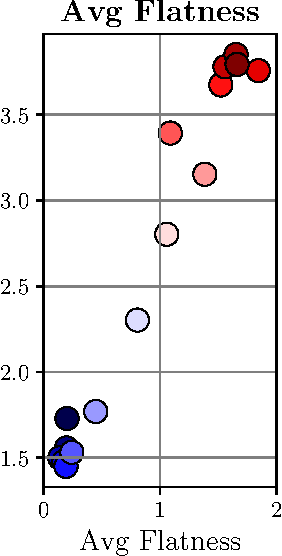
\includegraphics[height=3.5cm]{../paper/plots_main_flatness_epochs_correlation_seq}
				\end{minipage}
				\begin{minipage}[t]{0.25\textwidth}
					\vspace*{-2px}
					
					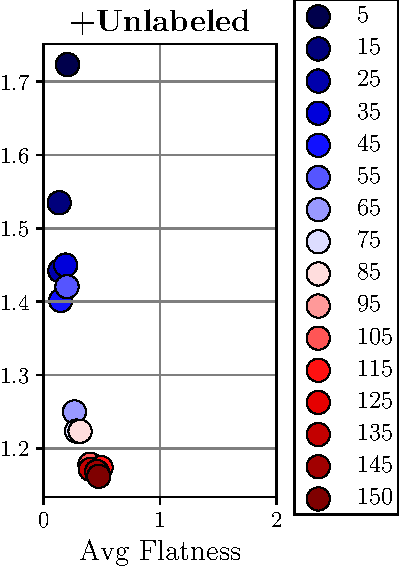
\includegraphics[height=3.5cm]{../paper/plots_main_flatness_epochs_correlation_seq_500k}
				\end{minipage}
			\end{center}
		\end{results}
		
		\begin{minipage}[t]{0.49\textwidth}
			\begin{problem}{\bf\large Conclusions}
				Robustness \emph{correlates} with flatness in RLoss:\\[1px]
				{\color{MPIIblue}$\RHD$} Robust overfitting reduces flatness.\\[1px]
				{\color{MPIIblue}$\RHD$} Popular AT variants find flatter minima.\\[1px]
				{\color{MPIIblue}$\RHD$} Optimizing flatness explicitly can improve robustness.
			\end{problem}
		\end{minipage}
		\begin{minipage}[t]{0.49\textwidth}
			\begin{results}{\bf\large Hyper-Parameters}
				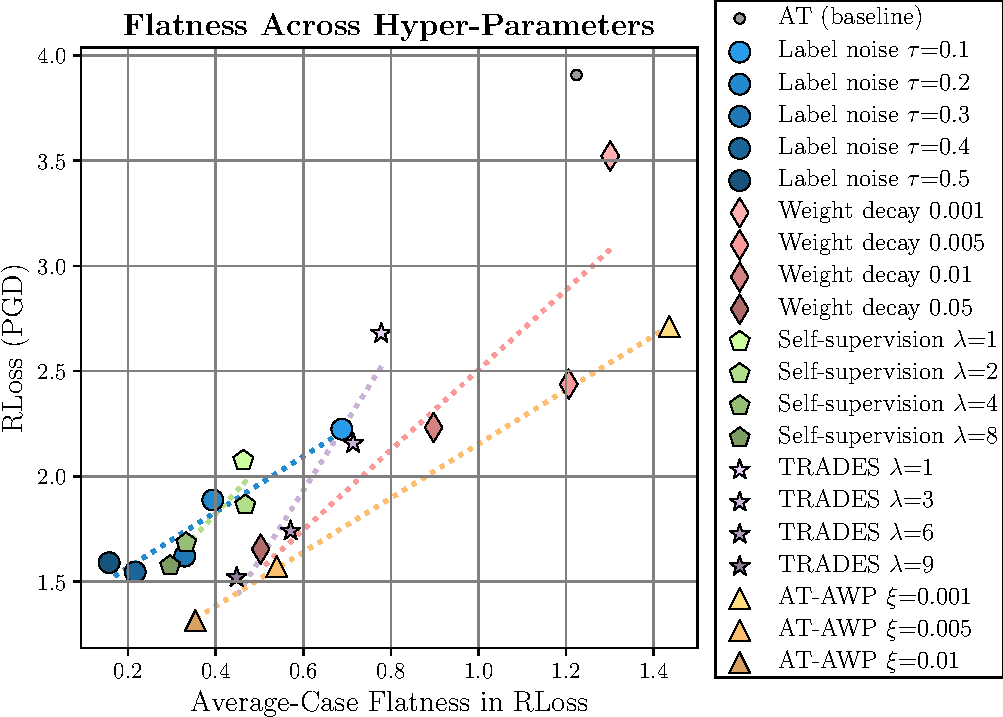
\includegraphics[width=1.01\textwidth]{../paper/plots_main_flatness_methods.pdf}
			\end{results}
		\end{minipage}
		
		\begin{results}{\bf\large Flatness and Robust Generalization}
			\begin{center}
				\begin{minipage}[t]{0.405\textwidth}
					\vspace*{0px}
					
					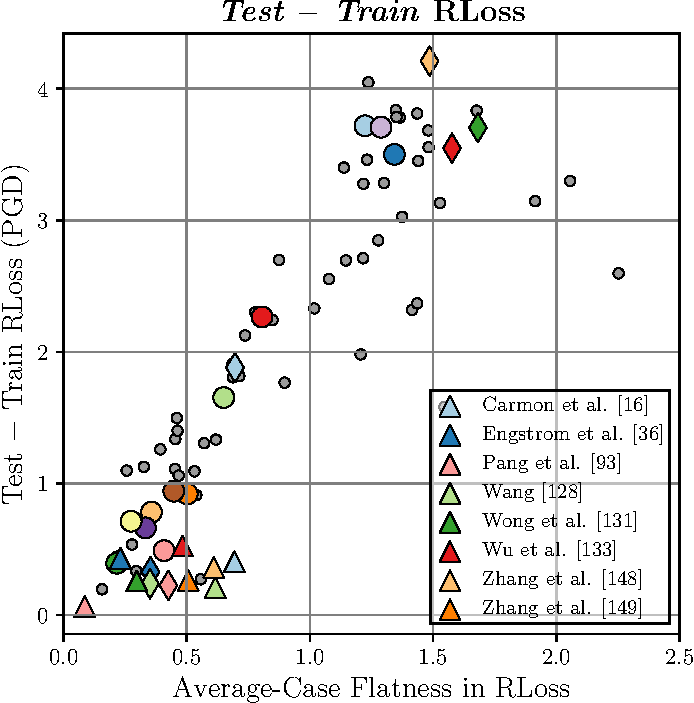
\includegraphics[width=1.025\textwidth]{../paper/plots_main_flatness_seq_test_train_arxiv.pdf}
				\end{minipage}
				\hfill
				\begin{minipage}[t]{0.405\textwidth}
					\vspace*{0px}
					
					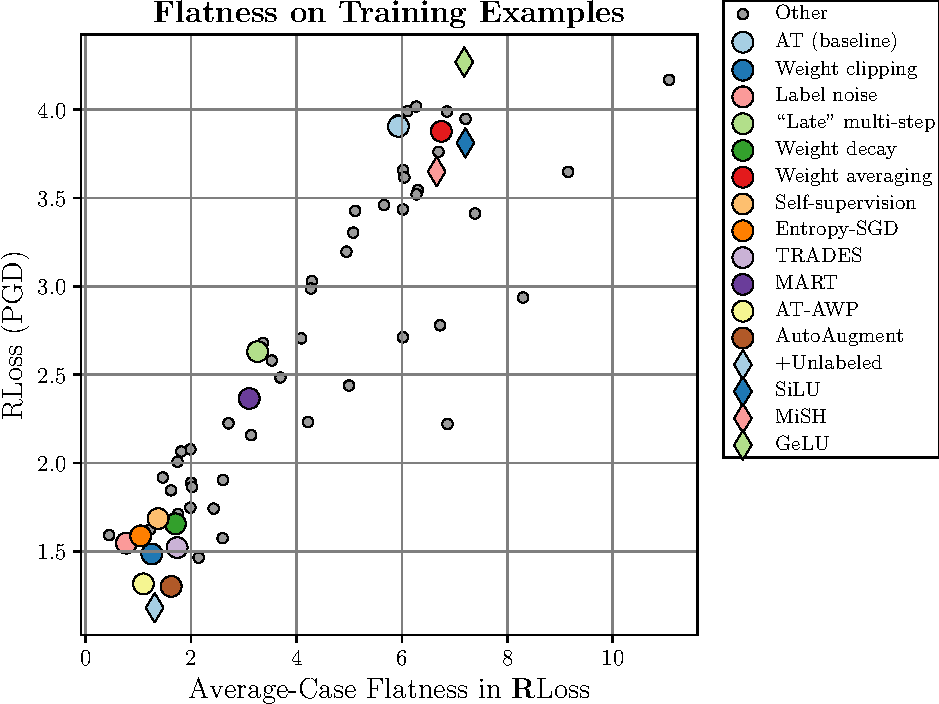
\includegraphics[width=1.025\textwidth,clip,trim={0 0 4.5cm 0}]{../paper/plots_supp_flatness_correlation_seq_train_loss.pdf}
				\end{minipage}
				\hfill
				\begin{minipage}[t]{0.16\textwidth}
					\vspace*{0px}
					
					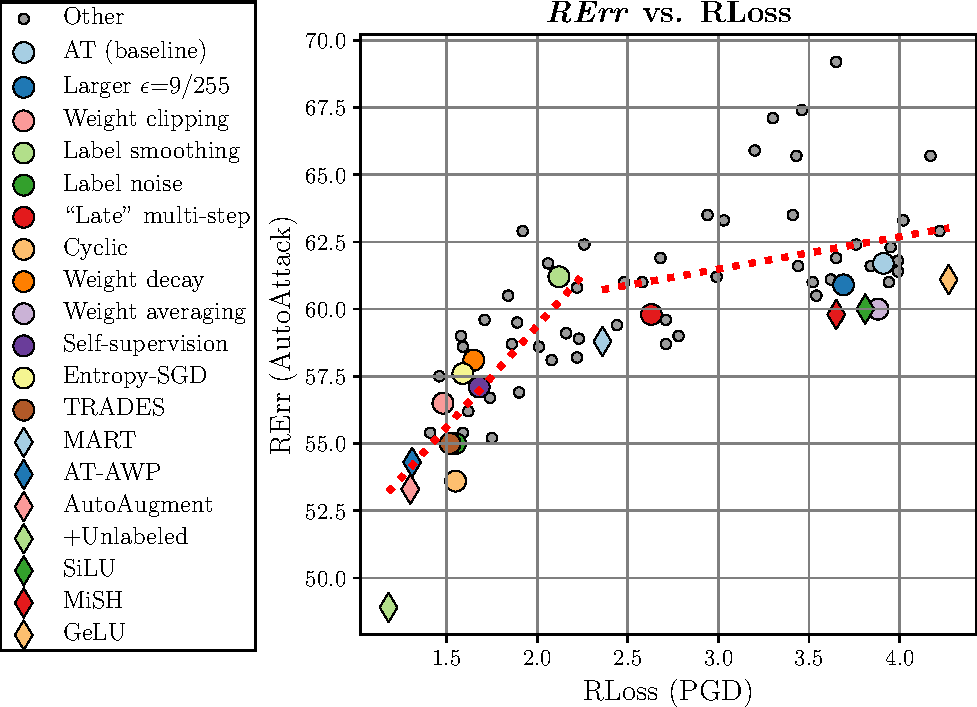
\includegraphics[width=\textwidth,clip,trim={0 0 12cm 0}]{../paper/plots_main_loss_error.pdf}
				\end{minipage}
			\end{center}
		\end{results}
    \end{minipage}
\end{document}
